 
%---------------------------------------------------------------------------
% Gui component.
%
%---------------------------------------------------------------------------


\section{GUI component}
\label{sec:arch_gui}

Graphical user interfaces are most commonly used form of interaction with user in modern computing. Designing decent
user interface is especially important due to aim of this work - creation of application allowing measuring and
visualization of monitored processes. Although GUI component has rather limited role of giving user control over
application and allow to view results of the work it's in fact most complex component. Additionally any shortcoming in
GUI is relatively difficult to be hidden by user, and that makes UI/UX (User Interface/User Experience) engineering so
important.

During designing user interface I've been trying to follow few general principles. First of all, I wanted used
interface to be as transparent as possible. Users should focus on their tasks instead of application. Because of that,
interface shouldn't be bloated with unnecessary options and steps that users need to achieve their goals should be as
short as possible. Next equally important interface item are visualizations. Because visualizations are most important
functionality of application, they need special concern. User should be able to view charts with results with out
any interruptions blocking or any other UI components that might be disturbing. What is also important, GUI must be
coherent to free user from chaos of being spread across multiple windows, desktops. 

From business logic point of view, GUI component will extensively use MVC design pattern\cite{gamma1995}. Each form,
window or more complex section need to have it's own View, responsible for presentation, Controller that collects
user's events and updates view on user's actions or system events. Application will have shared model, which will be
access point for underlaying components.
 


\subsection{Interface Mockups}

In this section, will try to describe mockups of most important views. The first mockup depicted in
Figure~\ref{fig:mock_main} shows main application view. Left edge of application window contains vertical tab pane
controller that will allow user to easily switch views covering 3 most important application contexts - resources,
measurements and visualizations. Another benefit of such a approach is that application has loads of space for what
user actually needs. The second most important component of main view is menu bar placed on top. It allows user
to perform bulk operations (e.g. pause all measurements) regardless of view he or she is currently. 

All subsequent mockups covers context specific views that will be rendered in main view's central pane.



\begin{figure}[ht]
  \centering
  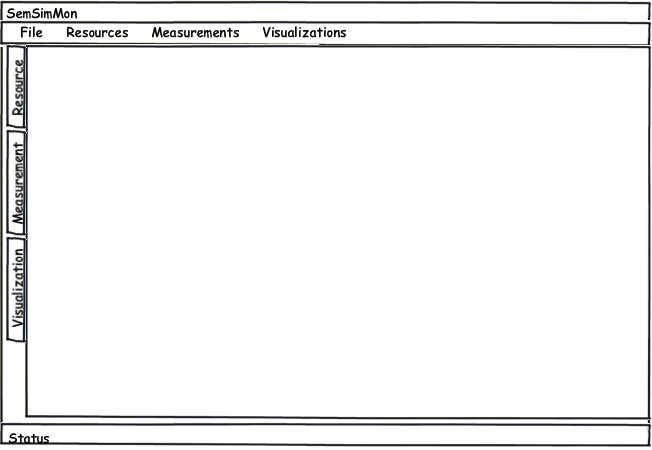
\includegraphics[width=0.7\textwidth]{mock_main}
  \caption{GUI application main view mockup}
  \label{fig:mock_main}
\end{figure}

When users starts to work with application He or She must add resources to be measured first. That's why resources view
is first, initial section shown to the user directly after page startup. Mockup of resources can bee seen in
Figure~\ref{fig:mock_resources}. The view is divided into 2 high level logical parts - the left pane covers global
resources context - users can browse measurement tree as well as add new resources into it. The right pane is specific
to resource selected by user and contains accordion with two sections. The upper one shows resource's static
attributes. The one below allow user to see snapshot of resource's dynamic state and check all of it's capabilities at
given point of time. To refresh those values, Refresh button was provided. Additionally, below accordion there are
several buttons allowing performing actions on given selected resource.

\begin{figure}[ht]
  \centering
  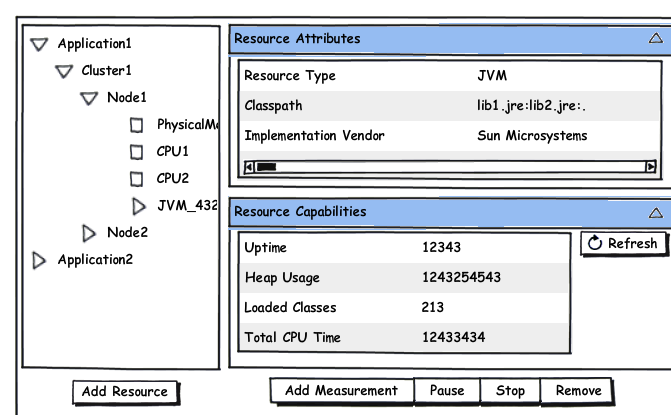
\includegraphics[width=0.7\textwidth]{mock_resources}
  \caption{GUI application resources pane}
  \label{fig:mock_resources}
\end{figure}

Next figure, Figure~\ref{fig:mock_measurements} covers measurements context of application. All measurements created
are listed on left side of this view. After selecting one accordion on right side shows details of selected
measurement. The upper section contain table with general informations. The lower one shows all measurement values
since the beginning. Additionally in this section user may copy the results into CSV format which can be easily
imported to spreadsheet application for further analysis. Using controls under measurements list, user can
pause, resume or remove measurement.

\begin{figure}[ht]
  \centering
  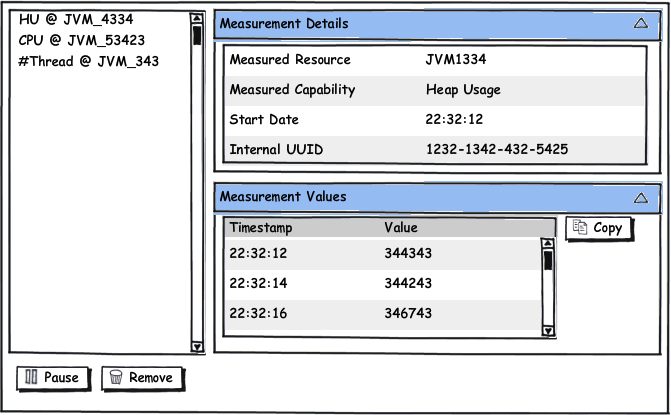
\includegraphics[width=0.7\textwidth]{mock_measurements}
  \caption{GUI application measurements pane}
  \label{fig:mock_measurements}
\end{figure}



\begin{figure}[ht]
  \centering
  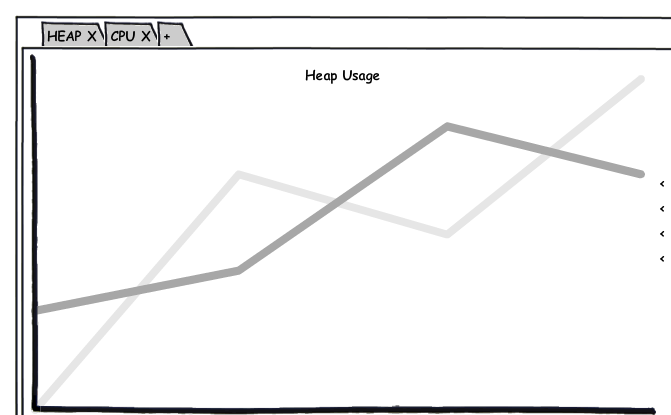
\includegraphics[width=0.7\textwidth]{mock_vis_clean}
  \caption{GUI application visualizations pane, clean view}
  \label{fig:mock_vis_clean}
\end{figure}

Appropriate visualizations display is probably most difficult for user experience engineering. During designing this UI
component I was inspiring myself from modest web browsers. The effects can be seen in Figure~\ref{fig:mock_vis_clean} -
in proposed solution every visualization is being rendered on separate, horizontal tab. To add new visualization, user
should just click last tab with appropriate icon. To remove visualization - user simply clicks cross icon on
visualization tab - just as He or She would close tab in browser. This gives visualization chart as much place as
application can give, and still allows user to easily control creation and disposal of visualization.

The biggest problem with such a approach is where to place controls of visualization. User must be able to choose which
measurements should be included in given visualization, as well as type of chart or other parameters. To address this
need, management pane was designed. It's hidden by default and is being displayed to the user, on mouse over right
edge of chart, marked with '<' signs. Layout of this pane is depicted in Figure~\ref{fig:mock_vis_options}. This
options pane contains form, divided into severals sections:

\begin{itemize}
 \item Visualization Options - user can here configure label of whole visualization, the one on tab pane
 \item Chart Options - allows setting chart's title (rendered on chart's graphics) and choose the chart type. User will
be able to use line (XY scatter), pie, bar and  spider web chart types.
 \item Measurements - gives control over which measurements should be included in given visualization. To add
measurement into visualization, user should click Add button and from displayed dialog choose which measurements should
be included. System doesn't give any constraints on measurements to be chosen, so it's up to the user to prepare
meaningful visualization. User will be able to remove given measurement from chart, by simply selecting it from list
and clicking Remove button.
 \item Actions - allows user to pause, resume visualization. Additionally user can copy to clipboard image containing
snapshot of visualization's chart.
\end{itemize}


\begin{figure}[ht]
  \centering
  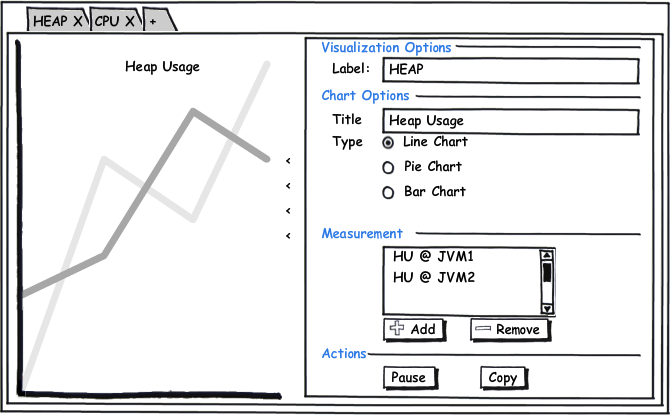
\includegraphics[width=0.7\textwidth]{mock_vis_options}
  \caption{GUI application visualizations pane, view with options pane}
  \label{fig:mock_vis_options}
\end{figure}



\subsection{Architecture}